\documentclass{article}
% This class needs 20 brownie points to get brownies!

% This document should have an example of everything covered in TeX in class on August 23, 2019.

% Title meta-data
\title{Math340 Day3}
\author{Zane and Dr. McNelis}
\date{23 August, 2019}

% Packages to load
\usepackage{marvosym} % For smiley face
\usepackage[margin=0.75in]{geometry} % Change margin size. See geometry documentation (CTAN) for all options.
\usepackage{graphicx} % Lets us put in pictures.

% Start document here
\begin{document}

\maketitle

\section{Smiley}
% In this section we want to print a smiley face symbol we found on DeTeXify.

% Needs the "marvosym" package for Smiley. See LaTeX cheat sheet on BlackBoard for more font size options.
\Huge{\Smiley}
\huge {\Smiley}

\section{More about tables.}
% In this section we will continue our discussion of the tabular environment from Yesterday.

% Placeholder options: c for center, l for left-justify, r for right-justify, p{width} for paragraph mode (forces a certain width on the column, wraps text downward).

\normalsize % Return text to original size.

% Movies table. Recall adding "|" (Shift-\) to placeholders makes lines. Adding \hline will print a horizontal line (as wide as the table).
\begin{tabular}{|l|c|p{3in}|}
\hline
\textbf{Movie} & \textbf{Year released} & \textbf{Description} \\
\hline
Movie 1 & 1974 & In this movie, there is a plot. \\
Movie 1: 2 (The sequel) & 1980 & This movie has a plot which is a sequel to the plot of Movie 1 (1974). \\
Movie 1/2 & 1999 & This movie shows the events which occurred after Movie 1, leading up to the plot of Movie 2. \\
\hline
\end{tabular}

\vspace{1cm}

% Advanced table techniques: rows spanning multiple columns. This is similar to merging cells in a spreadsheet. We will use \multicolumn{}{}{}, which is included in LaTeX by default.

% How \multicolumn works: \multicolumn{number of rows to merge}{alignment of merged cell -- bar/pipe can be included here}{text of the cell}

\begin{tabular}{c|c|c|c|c}
\multicolumn{2}{l|}{Name} & \multicolumn{2}{l|}{Info} & Housing \\
\hline
Last & First & Major & Standing & On/Off Campus \\
\hline
Billings & Zane & Math, Biology & Senior & On \\
McNelis & Erin & Math, Art & Super Senior & Off
\end{tabular}

\section{Getting pictures}
% You will need this package: 

% This is the most basic way to put in a picture.

\begin{center} % Recall that everything inside of this environment will be center-aligned. There is another way to center pictures we will discuss in the future.

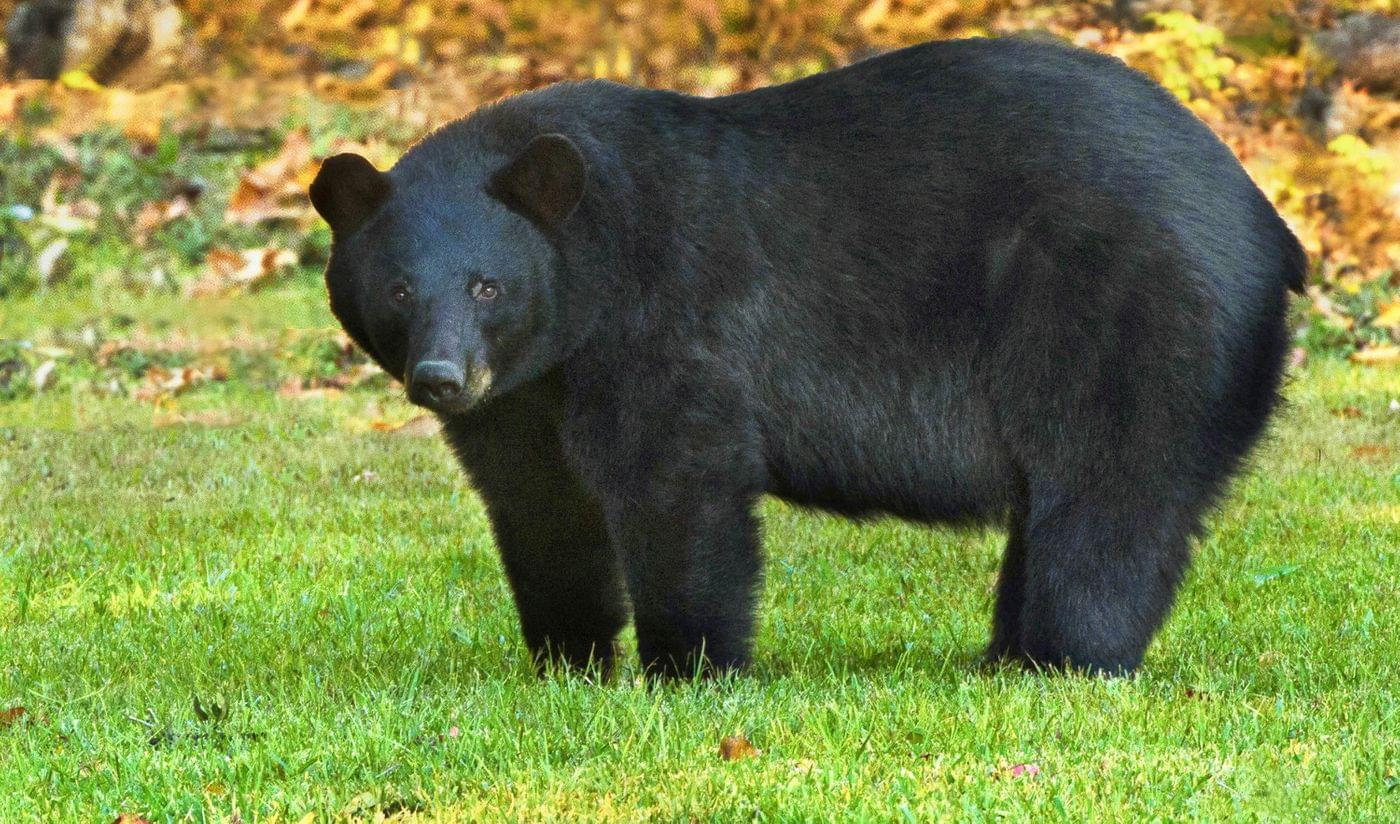
\includegraphics[width = 3in]{my_image.jpg} % You can specify the width, the height and other options in the square brackets. I wanted the picture to fit on the same page. See graphicx documentation (CTAN) or google for the rest of the options.

\end{center}

\end{document}





